\documentclass{retypeset}


\usepackage{tabularray}
\UseTblrLibrary{booktabs}
\UseTblrLibrary{diagbox}

\begin{document}
	
	
	%
	%第一册相关内容
	%
	
	%封面内容
	%\title{\Huge\bfseries 高中物理(甲种本)\\ 第一册 \vspace*{2cm} }
	%\author{\Large 张同恂 \and \Large 方玉珍 \and \Large 马淑美}
	%\date{\Large 1983年11月\\~\\~\\ \includegraphics[width=85mm]{fig/A/cover.pdf} }
	
	%\maketitle %封面
	%\tableofcontents %目录
	%\frontmatter
	%\chapter{说明}

本书是在中小学通用教材物理编写组编的
《全日制十年制学校高中课本(试用本)物理》的基础上,
按照高中物理教学大纲较高要求的内容编写成的.编
写中吸收了几年来各地试用中的一些经验和意见.许多省市的中学教师和有关
高等院校的教师对本书征求意见稿提了有益的意见和建议.北京、安徽、江西、
河南、上海、天津、浙江、江苏、湖北、广东、山西、黑龙江等省市的教研室
和教育学院在本书编写过程中给予了大力支持.在此谨致谢意.

希望广大教师和研究中学物理教学的同志提出批评和修改建议.
 %引言
	%\mainmatter
	
	
	%正文内容
	%\include{1/A/01} %力
	%\include{1/A/02} %直线运动
	%\include{1/A/03} %运动定律
	%\include{1/A/04} %曲线运动
	%\include{1/A/05} %万有引力定律
	%\include{1/A/06} %物体的平衡
	%\include{1/A/07} %机械能
	%\include{1/A/08} %动量
	%\include{1/A/09} %机械振动和机械波
	
	%\include{1/A/app_01} %学生实验
	%\chapter{课外实验活动}

\section{自制指南针}
如图~\ref{fig_C_10-10} 所示,用硬纸板、大头针、按扣、缝衣针自制一
个指南针.

用磁铁的一端在缝衣针上
朝一个方向擦几下,缝衣针就
有了磁性.为了使缝衣针能顺
利地穿过按扣(取按扣中较薄
的一扇)的两个小孔,可用钳子
把按扣的边缘向下夹一下,当
自制的指南针静下来后,记住针的哪一端指北.

\begin{figure}[htbp]
    \centering
    \includegraphics{fig/C/10-10.pdf}
    \caption{}\label{fig_C_10-10}
\end{figure}


\section{验证环形电流的磁场}
这个实验是用自制的指南针来验证环形电流的磁场方向
(图~\ref{fig_C_10-11}),在一个瓶子(或硬纸筒)上用漆包线绕一个10至15
匝的线圈,把绕好的线圈从瓶子上取下来,再用胶布把线圆竖
直固定在一块六板上,将你自制的指南针放在图~\ref{fig_C_10-11} 所示
的位置,转动木板使磁针处在线圈平面内,用学过的环形电
流磁场的知识判断一下,如果线圈的两端接上电池,指南针将
怎样偏转,然后再给线圈通电,看一看实验结果跟你的判断
是否一致.
\begin{figure}[htbp]
    \centering
    \includegraphics{fig/C/10-11.pdf}
    \caption{}\label{fig_C_10-11}
\end{figure}

    \section{验证通电螺线管的南北极}
把漆包线绕在一支铅笔上,然后抽出铅笔,做成一个螺线
管.用学过的通电螺线管磁场的知识判断一下,如果给螺线
管通电,通电螺线管哪端是南极,哪端是北极.然后把自制的
指南针放在螺线管的两端,给螺线管通电,看看实验结果跟你
的判断是否一致.

\section{观察磁化现象}
取一个条形磁铁和一个大铁钉,把铁钉插入铁屑,并把
条形磁铁的一个磁极靠近钉子头,然后同时提起磁铁和铁钉,
你将看到一些铁屑粘到钉子上.将磁铁移去,铁钉上的大部
分铁屑将掉下来,但仍有一部分铁屑粘在钉子上.再用磁铁
的另一个磁极靠近钉子头,剩在钉子上的铁屑就会掉下来.

解释上述现象.

\section{判断指南针的偏转方向}
在一个铅笔刀或一个大些的铁钉上,用漆包线绕上两个
线圈$A$和$B$,将线圈$B$的两端接在一起,并把$CD$段漆包线放
在静止的自制指南针的上方(图~\ref{fig_C_10-12}).试判断当用于电池
给线圈$A$通电的一瞬间,指南针偏转的方向.做这个实验,看
一看你判断的指南针偏转方向与实验是否一致.
\begin{figure}[htbp]
    \centering
    \includegraphics{fig/C/10-12.pdf}
    \caption{}\label{fig_C_10-12}
\end{figure}

\section{自制测电笔}
准备一个小氖灯,一个小弹簧,再找一个装中药片的小
玻璃瓶,两个瓶盖,两个铁钉,一个0.25瓦、2—5兆欧的电阻.
在稍粗糙的水泥砖上把玻璃瓶底磨掉,做成一个玻璃圆筒,让
铁钉穿过瓶盖,盖上瓶盖后使钉帽在瓶里,把电阻的两根引
线齐根去掉,并把电阻两端的绝缘漆去掉.照图~\ref{fig_C_10-13} 那样
把上述器材安装起来,就做成了一个测电笔.
\begin{figure}[htbp]
    \centering
    \includegraphics{fig/C/10-13.pdf}
    \caption{自制测电笔}\label{fig_C_10-13}
\end{figure}

用这个自制的测电笔可以辨别照明电路的火线和地线.
用拇指和食指拿住玻璃瓶,前面的钉子接触待辨别的导线,后
面的钉子接触手.当前面的钉子接触的是火线时,小氖灯发
光;接触的是地线时,小氖灯不发光.这样就可以辨别出火线
和地线.

要注意:\textit{手的任何部位都不要接触前面的钉子},因为它
接触可能是火线,会使人触电.

\section{测定水的折射率}
找一个广口瓶,在瓶内盛
满水,照图~\ref{fig_C_10-14} 那样把直尺$AB$
紧挨着瓶口的$C$点竖直插入瓶
内,从尺的对面一点$P$观察水
面,可以同时看到直尺在水中
的部分和露出水面的部分在水
中的像.读出你看到的直尺水
下部分最低点的刻度$S_1$,以及
跟这个刻度相重合的、水上部
分刻度$S_2$的像$S'_2$.记下$CS_1$和
$CS_2$的长度,量出广口瓶瓶口的内径$d$,就能算出水的折射率.
你用这种方法求出的水的折射率为多少?
 
如果你能同时读出直尺在水下的两个刻度$S_1$和$S_3$,以
及跟它们相重合的、两个水上刻度$S_2$和$S_4$在水中的像$S'_2$和
$S'_4$,就可以不必测量瓶口的内径,直接用从直尺上读出的两
组数据求出水的折射率来.比较这两种方法测量的结果,看
哪种方法测得的折射率更准确?

用后一种方法进行测量,瓶中的水不一定非盛满不可,竖
直插入水中的直尺也不一定要紧挨瓶口,做起来更简便.

\section{测定凹透镜的焦距}
凹透镜所成的虚像不能在像屏上显示出来,因此它的焦
距不可能象凸透镜那样直接利用焦点或成像方法来测量,
面介绍一种测量凹透镜焦距的简便方法.

\begin{figure}[htbp]
    \centering
    \begin{minipage}[t]{0.48\textwidth}
        \centering
        \includegraphics{fig/C/10-14.pdf}
        \caption{}\label{fig_C_10-14}
    \end{minipage}
    \begin{minipage}[t]{0.48\textwidth}
        \centering
        \includegraphics{fig/C/10-15.pdf}
        \caption{}\label{fig_C_10-15}
    \end{minipage}
\end{figure}



在凹透镜的中心贴一个半径为$R$的黑色圆纸片$A$,另取
一张白纸$B$,在$B$上画一个半径为$2R$的圆.把白纸和凹透镜
平行地放在太阳光下(图~\ref{fig_C_10-15}),让透镜对着太阳,调节透镜
和白纸间的距离,使黑色圆纸片的影恰好跟白纸上的圆圈重
合.这时透镜和白纸间的距离就等于凹透镜的焦距.想想看,
为什么?做这个实验,并将测得的焦距跟已知的焦距相比较,
看相差多少.




 %课外实验活动
	
	%\appendix
	%\chapter{国际单位制(SI)}

我们知道,物理公式在确定物理量的数量关系的同时,也
确定了物理量的单位关系.因此,只要我们选定为数不多的
几个物理量的单位,就能够利用它们推导出其他物理量的单
位.这些被任意选定的物理量叫做\textbf{基本量},如力学中的长度、
质量和时间就是三个基本量.
基本量的单位,如米、千克、秒
等,叫做\textbf{基本单位}.
由基本量根据有关公式推导出来的其他
物理量,叫做\textbf{导出量}.
导出量的单位叫做\textbf{导出单位}.


所谓单位制,就是有关基本单位、导出单位等一系列单位
的体制.
由于所采用的基本量的不同,基本单位的不同,以及
用来推导导出单位的定义公式的不同,存在着多种单位制.多
种单位制并用,给科学技术的交流和发展带来不便.
为了避免多种单位制的并存,国际上制订了一种通用的适合一切计
量领域的单位制,叫做国际单位制,国际代号为SI.国际单
位制是1960年第十一届国际计量大会通过的,其后并向全世
界推荐使用.
现在世界上许多国家采用了国际单位制或者正
在向国际单位制过渡,我国也统一实行以国际单位制为基础
的法定计量单位.

在力学范围内,国际单位制规定长度、质量和时间为三个
基本量,它们的单位用米、千克、秒为基本单位.
对于像热学、电磁学、光学等学科,除了上述三个基本单位外,还要加上另
外的基本量,并选定合适的基本单位,才能导出其他物理量的
单位.这样,国际单位制的基本单位共有七个.表~\ref{tab_A_10-4} 和表~\ref{tab_A_10-5} 分别列出了国际单位制的基本单位和常用的力学量的国际单
位制单位.

\begin{table}[htbp]
	\centering
	\caption{国际单位制的基本单位}\label{tab_A_10-4}
	\begin{tblr}{cccc}
		\hline
		\SetCell[r=2]{c} 物理量名称 & \SetCell[r=2]{c} 单位名称 & \SetCell[c=2]{c} 单位符号 \\
		&&中文 & 英文\\
		\hline
		长度 & 米 & 米 & m\\
		质量 & 千克 & 千克 &kg\\
		时间 & 秒 & 秒 &s\\
		电流 & 安培 & 安 &A\\ 
		热力学温度 & 开尔文 & 开 &K\\ 
		发光强度 & 坎德拉 & 坎 & cd\\
		物质的量 & 摩尔 & 摩 & mol\\
		\hline
	\end{tblr}
\end{table}

\begin{table}[htbp]
	\centering
	\caption{常用的力学量的国际单位制单位}\label{tab_A_10-5}
	{
	\zihao{5}
    \begin{tblr}{colspec={cc|ccc|c|c}}
        \hline
         \SetCell[c=2]{c} 物理量     & & \SetCell[c=3]{c} 单位 & & & \SetCell[r=2]{c} 量纲式 &  \SetCell[r=2]{c}备注\\
        名称 & 符号 & 名称 & 中文 & 英文 & & \\
        \hline
        面积    &  $S$    &  平方米    & $\text{米}^2$ & ${\rm m}^2$ & $[L^2]$ & \\
        体积   &  $V$    &   立方米   & $\text{米}^3$ &  ${\rm m}^3$ &$[L^3]$ & \\
        位移   &  $s$    &   米   & $\text{米}$ &  ${\rm m}$ &$[L]$ & \\
        速度   &   $v$   &    米每秒  & $\text{米}/\text{秒}$  & ${\rm m}/{\rm s}$ &$[LT^{-1}]$ &  \\
        加速度   &  $a$    & 米每二次方秒     & $\text{米}/\text{秒}^2$ &  ${\rm m}/{\rm s^2}$ & $[LT^{-2}]$ & \\
        角速度   &  $\omega$    &  弧度每秒    & $\text{弧度}/\text{秒}$ & ${\rm rad}/{\rm s}$ & $[T^{-1}]$ & \\
        角加速度   &  $d$    &   弧度每二次方秒   & $\text{弧度}/\text{秒}^2$ &  ${\rm rad}/{\rm s^2}$ & $[T^{-2}]$ & \\
        转速   &   $n$   &   1每秒   &  $1/\text{秒}$ &  ${\rm s}^{-1}$  & $[T^{-1}]$& \\
        频率   &  $\nu, f$    &  赫兹    & 赫 &  Hz & $[T^{-1}]$ & $1\text{赫}=1\text{秒}^{-1}$ \\
        密度   &  $\rho$    &  千克每立方米    & $\text{千克}/\text{米}^3$ & ${\rm kg}/{\rm m^3}$  &$[L^{-3}M]$ & \\
        力   &  $F$    &  牛顿    &  牛 &  N &$[LMT^{-2}]$ &  {$1\text{牛}=$\\$1 \text{千克}\cdot\text{米}/\text{秒}^2 $} \\
        重量   &  $G$    &    牛顿  &  牛 & N  &$[LMT^{-2}]$ & \\
        力矩   &  $M$    &    牛顿米  & $\text{牛}\cdot \text{米}$ & ${\rm N}\cdot {\rm m}$  & $[L^2MT^{-2}]$ & \\
        动量   &  $p$    & 千克米每秒    & $\text{千克}\cdot \text{米}/\text{秒}$ &  ${\rm kg}\cdot {\Ums}$ &$[LMT^{-1}]$ & \\
        冲量   &  $I$    &  牛顿秒    & $\text{牛}\cdot \text{秒}$ &   ${\rm N}\cdot {\rm s}$&$[LMT^{-1}]$ & \\
        压强   &  $p$    &   帕斯卡   &  帕  &  Pa & $[L^{-1}MT^{-2}]$ & $1 \text{帕} = 1 \text{牛}/\text{米}^2$ \\
        功   &  $W$    &   焦耳   & 焦 &  J & $[L^2MT^{-2}]$ & $1 \text{焦} = 1 \text{牛} \cdot \text{米}$ \\
        能   &   $E$   &   焦耳   & 焦 &  J & $[L^2MT^{-2}]$ & \\
        功率   &  $P$    &  瓦特    &  瓦  & W &$[L^2MT^{-3}]$ & $1\text{瓦}=1\text{焦}/\text{秒}$ \\
        \hline
    \end{tblr}
	}
\end{table}





\chapter{量纲}

我们知道,物理量可分为基本量和导出量.
既然导出量
可以从基本量导出,那么每个导出量一定可以用基本量的某
种组合表示出来.表示一个物理量是由哪些基本量组成和怎
样组成的式子,叫做这个物理量的\textbf{量纲式}.
在国际单位制中,
所有的力学量都是由长度、质量、时间这三个基本量组成的,
如果用$L $,$ M $,$ T$分别表示这三个基本量,那么,一个物理量$Q$
的量纲式的一般形式就是
\[[Q]=\qty[L^{\alpha}M^{\beta}T^{\gamma}]\]
其中$\alpha, \beta, \gamma$分别叫做物理量$Q$对于长度、质量、时间的\textbf{量纲}.

下面举出几个物理量的量纲式:
\begin{itemize}
    \item 体积的量纲式
    \[[V]=\qty[L^3]  \]
    \item 速度的量纲式
    \[[v]=\frac{[s]}{[t]}=\qty[LT^{-1}]  \] 
    \item 加速度的量纲式
    \[ [a]=\frac{[v]}{[t]}=\qty[LT^{-2}] \]
    \item 力的量纲式
    \[ [F]=[m][a]=\qty[LMT^{-2}] \]
\end{itemize}

在上面的表~\ref{tab_A_10-5} 中列出了一些力学量的量纲式.

物理量的量纲式可以用来检验物理关系式的正确性.检
验时所根据的原则是:只有量纲式相同的项才能相加减,而且
等号两边一定要有相同的量纲式.一个正确的物理关系式,
一定是符合上述原则的.






 %附录
	
	
	%
	%第二册相关内容
	%
	
	%封面内容
	%\title{\Huge\bfseries 高中物理(甲种本)\\ 第二册\vspace*{2cm}}
	%\author{\Large 张同恂\and \Large 方玉珍\and \Large 马淑美\and \Large 郭连壁\and \Large 李福利 }
	%\date{\Large 1984年7月 \\~\\~\\ \includegraphics[scale=1.2]{fig/B/cover.pdf}}
	
	%\maketitle %封面
	%\tableofcontents %目录
	%\frontmatter
	%\chapter{说明}

本书是在中小学通用教材物理编写组编的
《全日制十年制学校高中课本(试用本)物理》的基础上,
按照高中物理教学大纲较高要求的内容编写成的.编
写中吸收了几年来各地试用中的一些经验和意见.许多省市的中学教师和有关
高等院校的教师对本书征求意见稿提了有益的意见和建议.北京、安徽、江西、
河南、上海、天津、浙江、江苏、湖北、广东、山西、黑龙江等省市的教研室
和教育学院在本书编写过程中给予了大力支持.在此谨致谢意.

希望广大教师和研究中学物理教学的同志提出批评和修改建议.
 %说明
	%\mainmatter
	
	%正文内容
	%\include{1/B/01} %分子运动论基础
	%\include{1/B/02} %内能 能的转化和守恒定律
	%\include{1/B/03} %气体的性质
	%\include{1/B/04} %固体和液体的性质
	%\include{1/B/05} %物态变化
	\include{1/B/06} %电场
	%\include{1/B/07} %稳恒电流
	%\include{1/B/08} %物质的导电性
	
	%\include{1/B/app_01} %学生实验
	%\chapter{课外实验活动}

\section{自制指南针}
如图~\ref{fig_C_10-10} 所示,用硬纸板、大头针、按扣、缝衣针自制一
个指南针.

用磁铁的一端在缝衣针上
朝一个方向擦几下,缝衣针就
有了磁性.为了使缝衣针能顺
利地穿过按扣(取按扣中较薄
的一扇)的两个小孔,可用钳子
把按扣的边缘向下夹一下,当
自制的指南针静下来后,记住针的哪一端指北.

\begin{figure}[htbp]
    \centering
    \includegraphics{fig/C/10-10.pdf}
    \caption{}\label{fig_C_10-10}
\end{figure}


\section{验证环形电流的磁场}
这个实验是用自制的指南针来验证环形电流的磁场方向
(图~\ref{fig_C_10-11}),在一个瓶子(或硬纸筒)上用漆包线绕一个10至15
匝的线圈,把绕好的线圈从瓶子上取下来,再用胶布把线圆竖
直固定在一块六板上,将你自制的指南针放在图~\ref{fig_C_10-11} 所示
的位置,转动木板使磁针处在线圈平面内,用学过的环形电
流磁场的知识判断一下,如果线圈的两端接上电池,指南针将
怎样偏转,然后再给线圈通电,看一看实验结果跟你的判断
是否一致.
\begin{figure}[htbp]
    \centering
    \includegraphics{fig/C/10-11.pdf}
    \caption{}\label{fig_C_10-11}
\end{figure}

    \section{验证通电螺线管的南北极}
把漆包线绕在一支铅笔上,然后抽出铅笔,做成一个螺线
管.用学过的通电螺线管磁场的知识判断一下,如果给螺线
管通电,通电螺线管哪端是南极,哪端是北极.然后把自制的
指南针放在螺线管的两端,给螺线管通电,看看实验结果跟你
的判断是否一致.

\section{观察磁化现象}
取一个条形磁铁和一个大铁钉,把铁钉插入铁屑,并把
条形磁铁的一个磁极靠近钉子头,然后同时提起磁铁和铁钉,
你将看到一些铁屑粘到钉子上.将磁铁移去,铁钉上的大部
分铁屑将掉下来,但仍有一部分铁屑粘在钉子上.再用磁铁
的另一个磁极靠近钉子头,剩在钉子上的铁屑就会掉下来.

解释上述现象.

\section{判断指南针的偏转方向}
在一个铅笔刀或一个大些的铁钉上,用漆包线绕上两个
线圈$A$和$B$,将线圈$B$的两端接在一起,并把$CD$段漆包线放
在静止的自制指南针的上方(图~\ref{fig_C_10-12}).试判断当用于电池
给线圈$A$通电的一瞬间,指南针偏转的方向.做这个实验,看
一看你判断的指南针偏转方向与实验是否一致.
\begin{figure}[htbp]
    \centering
    \includegraphics{fig/C/10-12.pdf}
    \caption{}\label{fig_C_10-12}
\end{figure}

\section{自制测电笔}
准备一个小氖灯,一个小弹簧,再找一个装中药片的小
玻璃瓶,两个瓶盖,两个铁钉,一个0.25瓦、2—5兆欧的电阻.
在稍粗糙的水泥砖上把玻璃瓶底磨掉,做成一个玻璃圆筒,让
铁钉穿过瓶盖,盖上瓶盖后使钉帽在瓶里,把电阻的两根引
线齐根去掉,并把电阻两端的绝缘漆去掉.照图~\ref{fig_C_10-13} 那样
把上述器材安装起来,就做成了一个测电笔.
\begin{figure}[htbp]
    \centering
    \includegraphics{fig/C/10-13.pdf}
    \caption{自制测电笔}\label{fig_C_10-13}
\end{figure}

用这个自制的测电笔可以辨别照明电路的火线和地线.
用拇指和食指拿住玻璃瓶,前面的钉子接触待辨别的导线,后
面的钉子接触手.当前面的钉子接触的是火线时,小氖灯发
光;接触的是地线时,小氖灯不发光.这样就可以辨别出火线
和地线.

要注意:\textit{手的任何部位都不要接触前面的钉子},因为它
接触可能是火线,会使人触电.

\section{测定水的折射率}
找一个广口瓶,在瓶内盛
满水,照图~\ref{fig_C_10-14} 那样把直尺$AB$
紧挨着瓶口的$C$点竖直插入瓶
内,从尺的对面一点$P$观察水
面,可以同时看到直尺在水中
的部分和露出水面的部分在水
中的像.读出你看到的直尺水
下部分最低点的刻度$S_1$,以及
跟这个刻度相重合的、水上部
分刻度$S_2$的像$S'_2$.记下$CS_1$和
$CS_2$的长度,量出广口瓶瓶口的内径$d$,就能算出水的折射率.
你用这种方法求出的水的折射率为多少?
 
如果你能同时读出直尺在水下的两个刻度$S_1$和$S_3$,以
及跟它们相重合的、两个水上刻度$S_2$和$S_4$在水中的像$S'_2$和
$S'_4$,就可以不必测量瓶口的内径,直接用从直尺上读出的两
组数据求出水的折射率来.比较这两种方法测量的结果,看
哪种方法测得的折射率更准确?

用后一种方法进行测量,瓶中的水不一定非盛满不可,竖
直插入水中的直尺也不一定要紧挨瓶口,做起来更简便.

\section{测定凹透镜的焦距}
凹透镜所成的虚像不能在像屏上显示出来,因此它的焦
距不可能象凸透镜那样直接利用焦点或成像方法来测量,
面介绍一种测量凹透镜焦距的简便方法.

\begin{figure}[htbp]
    \centering
    \begin{minipage}[t]{0.48\textwidth}
        \centering
        \includegraphics{fig/C/10-14.pdf}
        \caption{}\label{fig_C_10-14}
    \end{minipage}
    \begin{minipage}[t]{0.48\textwidth}
        \centering
        \includegraphics{fig/C/10-15.pdf}
        \caption{}\label{fig_C_10-15}
    \end{minipage}
\end{figure}



在凹透镜的中心贴一个半径为$R$的黑色圆纸片$A$,另取
一张白纸$B$,在$B$上画一个半径为$2R$的圆.把白纸和凹透镜
平行地放在太阳光下(图~\ref{fig_C_10-15}),让透镜对着太阳,调节透镜
和白纸间的距离,使黑色圆纸片的影恰好跟白纸上的圆圈重
合.这时透镜和白纸间的距离就等于凹透镜的焦距.想想看,
为什么?做这个实验,并将测得的焦距跟已知的焦距相比较,
看相差多少.




 %课外实验活动
	
	%\appendix
	%\chapter{常用的热学量和电学量的国际单位制单位}

\begin{table}[htbp]
    \centering
    \begin{tabular}{cc|cc|c|c}
        \toprule
        \multicolumn{2}{c|}{物理量} & \multicolumn{2}{c|}{单位} & 量纲式 & 备注\\
        名称&符号 &中文符号&英文符号& & \\
        \midrule
        热力学温度      &   $T$               &    开      &    K  &  $[\Theta]$  & \\
        热量      &   $Q$             &     焦     &    J  &  $[L^2MT^{-2}]$ & \\
        比热      &   $c$             &  焦/千克$\cdot $开        & J/(kg$\cdot$K)  & $[L^2T^{-2}\Theta^{-1}]$ & \\  
        电流      &    $I$             &   安       &    A & $[I]$ & \\
        电量      &    $Q$            &    库      &    C & $[TI]$ & $1  \text{ 库}=1 \text{ 安} \cdot \text{秒} $ \\
        电场强度      &  $E$              &  伏/米$^2$        &   V/m$^2$  & $[LMT^{-3}I^{-1}]$ & \\
        电势(差)、电压      & $U(V)$              &    伏      &   V  & $[L^2MT^{-3}I^{-1}]$ & $ 1 \text{ 伏} = 1 \text{ 瓦}/\text{安} $\\
        电动势      &  $\mathcal{E}$              &    伏      &    V & $[L^2MT^{-3}I^{-1}]$ & \\
        电容      &    $C$          &    法      &   F  & $[L^{-2}M^{-1}T^{4}I^{2}]$ & $1 \text{ 法} = 1 \text{ 库}/\text{伏}$ \\
        电阻      &    $R$        &     欧     &    $\Omega$       & $[L^{2}MT^{-3}I^{-2}]$ & $1 \text{ 欧}=1 \text{ 伏}/\text{安}$ \\
        电阻率      &    $\rho$          &   欧$\cdot$米       & $\Omega\cdot{\rm m}$   &  $[L^{3}MT^{-3}I^{-2}]$ & \\
        \bottomrule
    \end{tabular}
\end{table}

 %附录
	
	
	%
	%第三册相关内容
	%
	
	%封面内容
	%\title{\Huge\bfseries 高中物理(甲种本)\\ 第三册\vspace*{2cm} }
	%\author{\Large 张同恂\and \Large 方玉珍\and \Large 马淑美}
	%\date{\Large 1985年11月\\~\\~\\ \includegraphics[scale=1.8]{fig/C/cover.pdf}}
	
	%\maketitle %封面
	%\tableofcontents %目录
	%\frontmatter
	%\chapter{说明}

本书是在中小学通用教材物理编写组编的
《全日制十年制学校高中课本(试用本)物理》的基础上,
按照高中物理教学大纲较高要求的内容编写成的.编
写中吸收了几年来各地试用中的一些经验和意见.许多省市的中学教师和有关
高等院校的教师对本书征求意见稿提了有益的意见和建议.北京、安徽、江西、
河南、上海、天津、浙江、江苏、湖北、广东、山西、黑龙江等省市的教研室
和教育学院在本书编写过程中给予了大力支持.在此谨致谢意.

希望广大教师和研究中学物理教学的同志提出批评和修改建议.
 %说明
	%\mainmatter
	
	%正文内容
	%\include{1/C/01} %磁场
	%\include{1/C/02} %电磁感应
	%\include{1/C/03} %交流电
	%\include{1/C/04} %电磁振荡和电磁波
	%\include{1/C/05} %光的反射和折射
	%\include{1/C/06} %光的波动性
	%\include{1/C/07} %光的粒子性
	%\include{1/C/08} %原子结构
	%\include{1/C/09} %原子核
	
	%\include{1/C/app_01} %学生实验
	%\chapter{课外实验活动}

\section{自制指南针}
如图~\ref{fig_C_10-10} 所示,用硬纸板、大头针、按扣、缝衣针自制一
个指南针.

用磁铁的一端在缝衣针上
朝一个方向擦几下,缝衣针就
有了磁性.为了使缝衣针能顺
利地穿过按扣(取按扣中较薄
的一扇)的两个小孔,可用钳子
把按扣的边缘向下夹一下,当
自制的指南针静下来后,记住针的哪一端指北.

\begin{figure}[htbp]
    \centering
    \includegraphics{fig/C/10-10.pdf}
    \caption{}\label{fig_C_10-10}
\end{figure}


\section{验证环形电流的磁场}
这个实验是用自制的指南针来验证环形电流的磁场方向
(图~\ref{fig_C_10-11}),在一个瓶子(或硬纸筒)上用漆包线绕一个10至15
匝的线圈,把绕好的线圈从瓶子上取下来,再用胶布把线圆竖
直固定在一块六板上,将你自制的指南针放在图~\ref{fig_C_10-11} 所示
的位置,转动木板使磁针处在线圈平面内,用学过的环形电
流磁场的知识判断一下,如果线圈的两端接上电池,指南针将
怎样偏转,然后再给线圈通电,看一看实验结果跟你的判断
是否一致.
\begin{figure}[htbp]
    \centering
    \includegraphics{fig/C/10-11.pdf}
    \caption{}\label{fig_C_10-11}
\end{figure}

    \section{验证通电螺线管的南北极}
把漆包线绕在一支铅笔上,然后抽出铅笔,做成一个螺线
管.用学过的通电螺线管磁场的知识判断一下,如果给螺线
管通电,通电螺线管哪端是南极,哪端是北极.然后把自制的
指南针放在螺线管的两端,给螺线管通电,看看实验结果跟你
的判断是否一致.

\section{观察磁化现象}
取一个条形磁铁和一个大铁钉,把铁钉插入铁屑,并把
条形磁铁的一个磁极靠近钉子头,然后同时提起磁铁和铁钉,
你将看到一些铁屑粘到钉子上.将磁铁移去,铁钉上的大部
分铁屑将掉下来,但仍有一部分铁屑粘在钉子上.再用磁铁
的另一个磁极靠近钉子头,剩在钉子上的铁屑就会掉下来.

解释上述现象.

\section{判断指南针的偏转方向}
在一个铅笔刀或一个大些的铁钉上,用漆包线绕上两个
线圈$A$和$B$,将线圈$B$的两端接在一起,并把$CD$段漆包线放
在静止的自制指南针的上方(图~\ref{fig_C_10-12}).试判断当用于电池
给线圈$A$通电的一瞬间,指南针偏转的方向.做这个实验,看
一看你判断的指南针偏转方向与实验是否一致.
\begin{figure}[htbp]
    \centering
    \includegraphics{fig/C/10-12.pdf}
    \caption{}\label{fig_C_10-12}
\end{figure}

\section{自制测电笔}
准备一个小氖灯,一个小弹簧,再找一个装中药片的小
玻璃瓶,两个瓶盖,两个铁钉,一个0.25瓦、2—5兆欧的电阻.
在稍粗糙的水泥砖上把玻璃瓶底磨掉,做成一个玻璃圆筒,让
铁钉穿过瓶盖,盖上瓶盖后使钉帽在瓶里,把电阻的两根引
线齐根去掉,并把电阻两端的绝缘漆去掉.照图~\ref{fig_C_10-13} 那样
把上述器材安装起来,就做成了一个测电笔.
\begin{figure}[htbp]
    \centering
    \includegraphics{fig/C/10-13.pdf}
    \caption{自制测电笔}\label{fig_C_10-13}
\end{figure}

用这个自制的测电笔可以辨别照明电路的火线和地线.
用拇指和食指拿住玻璃瓶,前面的钉子接触待辨别的导线,后
面的钉子接触手.当前面的钉子接触的是火线时,小氖灯发
光;接触的是地线时,小氖灯不发光.这样就可以辨别出火线
和地线.

要注意:\textit{手的任何部位都不要接触前面的钉子},因为它
接触可能是火线,会使人触电.

\section{测定水的折射率}
找一个广口瓶,在瓶内盛
满水,照图~\ref{fig_C_10-14} 那样把直尺$AB$
紧挨着瓶口的$C$点竖直插入瓶
内,从尺的对面一点$P$观察水
面,可以同时看到直尺在水中
的部分和露出水面的部分在水
中的像.读出你看到的直尺水
下部分最低点的刻度$S_1$,以及
跟这个刻度相重合的、水上部
分刻度$S_2$的像$S'_2$.记下$CS_1$和
$CS_2$的长度,量出广口瓶瓶口的内径$d$,就能算出水的折射率.
你用这种方法求出的水的折射率为多少?
 
如果你能同时读出直尺在水下的两个刻度$S_1$和$S_3$,以
及跟它们相重合的、两个水上刻度$S_2$和$S_4$在水中的像$S'_2$和
$S'_4$,就可以不必测量瓶口的内径,直接用从直尺上读出的两
组数据求出水的折射率来.比较这两种方法测量的结果,看
哪种方法测得的折射率更准确?

用后一种方法进行测量,瓶中的水不一定非盛满不可,竖
直插入水中的直尺也不一定要紧挨瓶口,做起来更简便.

\section{测定凹透镜的焦距}
凹透镜所成的虚像不能在像屏上显示出来,因此它的焦
距不可能象凸透镜那样直接利用焦点或成像方法来测量,
面介绍一种测量凹透镜焦距的简便方法.

\begin{figure}[htbp]
    \centering
    \begin{minipage}[t]{0.48\textwidth}
        \centering
        \includegraphics{fig/C/10-14.pdf}
        \caption{}\label{fig_C_10-14}
    \end{minipage}
    \begin{minipage}[t]{0.48\textwidth}
        \centering
        \includegraphics{fig/C/10-15.pdf}
        \caption{}\label{fig_C_10-15}
    \end{minipage}
\end{figure}



在凹透镜的中心贴一个半径为$R$的黑色圆纸片$A$,另取
一张白纸$B$,在$B$上画一个半径为$2R$的圆.把白纸和凹透镜
平行地放在太阳光下(图~\ref{fig_C_10-15}),让透镜对着太阳,调节透镜
和白纸间的距离,使黑色圆纸片的影恰好跟白纸上的圆圈重
合.这时透镜和白纸间的距离就等于凹透镜的焦距.想想看,
为什么?做这个实验,并将测得的焦距跟已知的焦距相比较,
看相差多少.




 %课外实验活动
	
	%\appendix
	%\chapter{常用电磁学量的国际制单位}

电磁学的单位制是一个比较复杂的问题.
长期以来存在着多种单位制.
本书采用的是国际单位制.在国际单位制中,
所有的电磁学量,都是由长度、质量、时间、电流强度这四个基
本量导出的.因此,米、千克、秒、安培是电磁学里的基本单位.
表~\ref{tab_C_10-1} 列出了常用的电磁学量的国际制单位.

\begin{table}[htbp]
	\centering
	\caption{}\label{tab_C_10-1}
	{
	\zihao{5}
    \begin{tblr}{colspec={cc|ccc|c|c}, cell{1}{1}={c=2}{c}, cell{1}{3}={c=3}{c},cell{1}{6}={r=2}{c},cell{1}{7}={r=2}{c},cells={valign=m},cell{6}{1-Z}={bg=gray!40}}
  		\toprule
		物理量& & 单位 & && 量纲式 & 备注\\
		名称 & 符号 & 名称 &中文符号& 英文符号 & & \\
		  \midrule
		电流   &  $I$ & 安培 &安& $\UA$ & $[I]$ & \\
		电量    &  $Q$  &  库仑  &库& $\UC$   & $[TI]$  &  $1 \text{ 库}=1\text{ 安}\cdot \text{秒}$\\
		电场强度    &$E$    &  伏特每米  &伏/米& $\UVm$   &  $[LMT^{-3}I^{-1}]$  & \\
		{电势、电压\\电势差} & $U(V)$  &  伏特  &伏&  $\UV$  &  $[L^2MT^{-3}I^{-1}]$ & $1 \text{ 伏} =1 \text{ 瓦}/\text{安}$ \\
		电容    &  $C$  &  法拉  &法& $\UF$   &  $[L^{-2}M^{-1}T^{4}I^{2}]$  & $1 \text{ 法}=1 \text{ 库}/\text{伏}$ \\
		电阻    & $R$  & 欧姆  &欧&  $\UO$ & $[L^2MT^{-3}I^{-2}]$  & $1 \text{ 欧}=1 \text{ 伏}/\text{安}$ \\
		电阻率    & $\rho$  & 欧姆米  &欧$\cdot$米&  $\UOm$ & $[L^3MT^{-3}I^{-2}]$  & \\
		磁感应强度    & $B$  & 特斯拉  &特& $\UT$  &  $[MT^{-2}I^{-1}]$ & $1 \text{ 特}=1 \text{ 韦}/\text{米}^2$ \\
		磁通量    & $\phi$  & 韦伯  &韦& $\UWb$  & $[L^2MT^{-2}I^{-1}]$ & $1 \text{ 韦}=1 \text{ 伏}\cdot\text{秒}$ \\
		电感    & $L$  & 亨利  &享& $\UH$  &  $[L^2MT^{-2}I^{-2}]$ & $1 \text{ 享}=1 \text{ 韦}/\text{安}$ \\
		  \bottomrule   
    \end{tblr}
	}
\end{table}

\chapter{常用的物理恒量}
\begin{table}[htbp]
	\centering
	\caption{}\label{tab_C_10-2}
    \begin{tblr}{rl}
        万有引力恒量&    $G=6.67\times10^{-11} \UNmqkgq$\\
        摩尔气体恒量&    $R=8.31 \UJmolK $\\
        阿伏伽德罗常数&    $N=6.02\times 10^{23} \Umoln$\\
        静电力恒量&    $k=9.0\times10^9 \UNmqCq $\\
        法拉第恒量&    $F=9.65\times10^4 \UCmol$\\
        基本电荷&    $e=1.60\times10^{-19} \UC$\\
        电子的质量&    $m_e=0.91\times10^{-30} \Ukg$\\
        质子的质量&    $m_p=1.67\times10^{-27} \Ukg$\\
        中子的质量&    $m_n=1.67\times10^{-27} \Ukg$\\
        $\alpha$粒子的质量&    $m_{\alpha}=6.64\times10^{-27} \Ukg$\\
        原子质量单位&    $1{\rm u}=1.66\times10^{-27} \Ukg $\\
        真空中光速&    $c=3.00\times10^8 \Ums$\\
        电子的荷质比&    $e/m=1.76\times10^{11} \UCkg $ \\
        氢原子的半径&    $a_0=0.53\times10^{-10} \Um $   \\
        普朗克恒量&    $h=6.63\times10^{-34} \UJcdots$   \\
        里德伯恒量&    $R=1.097\times10^7 \Umn$\\        
    \end{tblr}
\end{table}

\chapter{用于构成十进倍数和分数单位的词头}

\begin{table}[htbp]
	\centering
	\caption{}\label{tab_C_10-3}
    \begin{tblr}{colspec={cccc},cells={valign=m}}
        \toprule
		所表示的因数&{词头名称\\(中文)}&{词头名称\\(英文)}&词头符号\\
		\midrule
		$10^{18}$ &艾[可萨]&exa-&E\\
		$10^{15}$ &拍[它]&peta-&P\\
		$10^{12}$ &太[拉]&tera-&T\\
		$10^9$ &吉[咖] &giga-&G\\
		$10^6$ &兆 &mega-&M\\
		$10^3$ & 千 &kilo-& k\\
		$10^2$ & 百 &hecto-&h\\
		$10^1$ & 十 &deca-&da\\
		$10^{-1}$ & 分 &deci-&d\\
		$10^{-2}$ &厘 &centi-&c\\
		$10^{-3}$ &毫 &milli-&m\\
		$10^{-6}$&微&micro-&$\mu$\\
		$10^{-9}$&纳[诺]  &nano-&n\\
		$10^{-12}$ &皮[可]&pico-&p\\
		$10^{-15}$&飞[母托]&femto-&f\\
		$10^{-18}$&阿[托]&atto-&a\\
		\bottomrule
    \end{tblr}
\end{table}



 %附录
	
\end{document}


